\documentclass[a4paper,14pt]{article}
\usepackage[T1]{fontenc}
\usepackage[utf8]{inputenc}
\usepackage{lmodern}
\usepackage{amsmath}
\usepackage{amsfonts}
\usepackage{amssymb}
\usepackage{amsthm}
\usepackage{graphicx}
\usepackage{color}
\usepackage{xcolor}
\usepackage{url}
\usepackage{textcomp}
\usepackage{parskip}
\usepackage{pdfpages}
\usepackage{hyperref}
\usepackage{float}
\usepackage{enumitem}
\usepackage{subfig}
\usepackage{fancyhdr}

\renewcommand{\figurename}{Slika}
\graphicspath{ {./img/} }

\title{Operativni sistem Linux}
\author{Aleksa Siriški}
\date{May 2022}

\begin{document}

\pagestyle{empty}
\begin{center}
\textbf{Gimnanzija „Jovan Jovanović Zmaj“}
\\
Novi Sad
\end{center}
\vfill
\begin{center}
	\begin{large}
		\textbf{Maturski rad iz Operativnih Sistema}
		\bigskip 
	\end{large}
	\\
	\begin{huge}
        \textbf{Operativni sistem Linux}
	\end{huge}
\end{center}
\vfill
\begin{normalsize}
Profesor mentor:
\hfill
Učenik:
\\
Saša Tošić
\hfill
Aleksa Siriški IV-6
\end{normalsize}
\vfill
\begin{center}
Novi Sad, maj 2022. god.
\end{center}
\newpage

\pagestyle{plain}
\section{Predgovor}
Za ovu temu sam se opredelio iz više razloga. Prvenstveno zbog ljubavi prema informacionim tehnologijama, koju sam stekao zahvaljujući mojim roditeljima. Drugi razlog je to što smatram da je ovo veoma fascinantna tema, jer obuhvata kompleksnost koje se može postići kada na jednom projektu radi čitav svet. Na kraju, ono što me je privuklo da izaberem baš ovu temu, jeste činjenica da je budućnost IT-a slobodan i besplatan kod.
\\\\
U ovom radu, analiziraću osnovne komponente jednog izuzetnog operativnog sistema, istoriju njegove kreacije kao i filozofski pogled na isti.
\newpage

\renewcommand{\contentsname}{Sadržaj}
\tableofcontents
\newpage

\pagestyle{fancy}
\fancyhf{}
\lhead{Operativni sistem Linux}
\rhead{Aleksa Siriški, IV-6}
\cfoot{\thepage}

\section{Istorija}
Unix su stvorili i objavili Ken Thompson i Dennis Ritchie 1970. godine. Kasnije je prekucan u C programskom jeziku i time postao veoma fleksibilan i izmenljiv. Razni fakulteti i univerziteti su pravili svoje verzije Unix-a, npr. BSD koji je nalik Linuxa i dan danas u upotrebi.
\\\\
Richard Matthew Stallman, osnivač GNU projekta, je uz svoj tim započeo izradu kompletnog operativnog sistema čija je glavna namena da bude otvorena i slobodna alternativa za Unix. Jedina stvar koja je falila jeste kernel, sto je jezgro operativnog sistema koje služi da poveže sve druge komponente u zajednicu.
\\\\
Linus Torvalds koji je bio iznerviran nedostatkom kernela za potpuno slobodan i otvoren operativni sistem odlučuje da napiše svoj sopstveni. Već je bio upućen u Minix i GNU softver te je tokom studija u Finskoj započeo projekat nazvan "Linux". U početku je jedini radio na njemu, ali do danas se priključilo preko 15000 programera u kreiranju kernela koji se sastoji iz vise od 17 miliona linija koda.
\\\\
\begin{figure}[h]
	\centering
    \subfloat[Ken Thompson i Dennis Ritchie, tvorci Unix-a]{{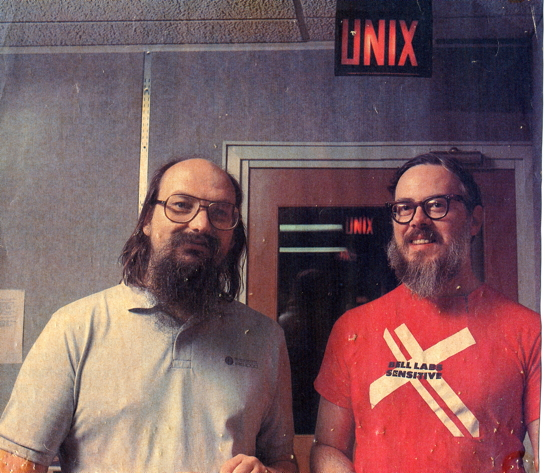
\includegraphics[height=3cm,width=4cm]{ken-thompson-dennis-ritchie} }}
    \hspace{1cm}
    \subfloat[Linus Torvalds, tvorac Linux-a]{{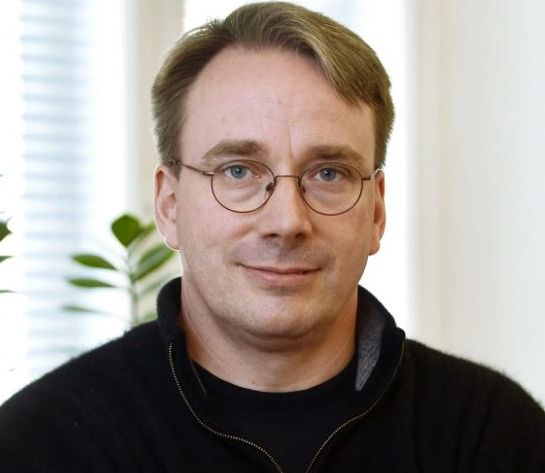
\includegraphics[height=3cm,width=4cm]{linus-torvalds} }}
\end{figure}
\begin{figure}[h]
	\centering
    \subfloat[Linux]{{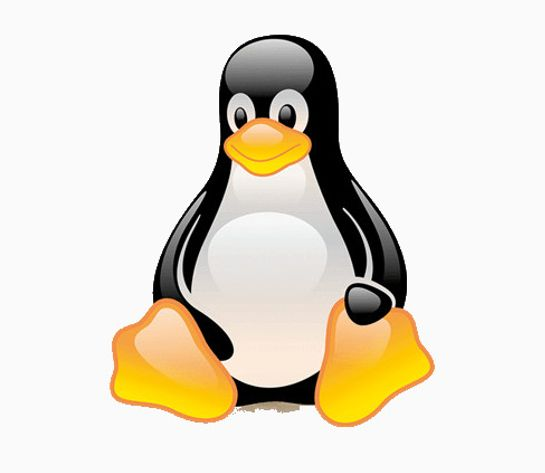
\includegraphics[height=3cm,width=4cm]{linux} }}
    \hspace{1cm}
    \subfloat[Richard Matthew Stallman, tvorac GNU-a]{{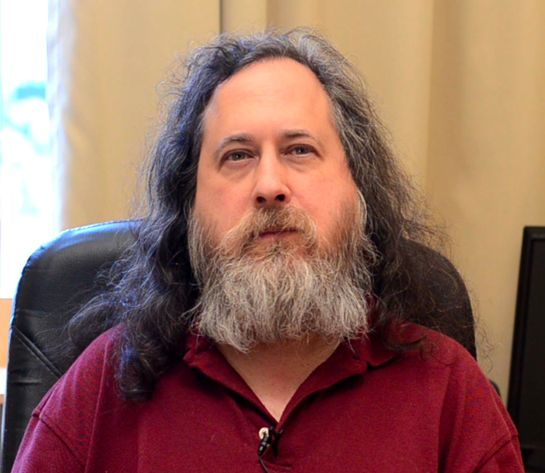
\includegraphics[height=3cm,width=4cm]{richard-stallman} }}
\end{figure}
\newpage

\section{Komponente}
\subsection{Distribucije}
GNU/Linux operativni sistem se može samostalno napraviti od nule, kompajliranjem svih potrebnih programa (npr. Linux From Scratch), ali se najčešće koriste već gotove distribucije. Sve distribucije dele jednu stvar, Linux kernel, ali po svemu drugom se mogu potpuno razlikovati, doduše većina distribucija ima neke zajedničke osnovne komponente.
\\\\
Postoje distribucije pravljene za servere:
\begin{itemize}
\item Debian
\item Ubuntu server
\item CentOS
\item Turnkey
\end{itemize}
Kao i distribucije pravljene za desktop korisnike:
\begin{itemize}
\item Ubuntu
\item Linux Mint
\item PopOS
\item Fedora Workstation
\end{itemize}
Takođe postoje minimalne distribucije pravljene za kontejnere:
\begin{itemize}
\item Alpine Linux
\item Fedora CoreOS
\item openSUSE MicroOS
\end{itemize}
\newpage
\subsection{Kernel}
Kernel je najvažniji deo svakog operativnog sistema. Služi da pokrene svaku komponentu koja je potrebna za korišćenje OS-a kao i da dozvoli komunikaciju softvera sa hardverom, ili jednog softvera sa drugim. Kernel je neophodan da bi operativni sistem funkcionisao i kao takav je ključno da je minimalan i efikasan.
\\\\
Osnovni delovi kernela su:
\begin{itemize}
\item Menadžer procesa - kao što mu ime implicira služi da rukuje procesima tj. programima. Svaki proces je zapravo svoj virtualni procesor, nazvan nit (eng. thread). Programi mogu alocirati više niti, zvani radnici (eng. workers). Termin proces i nit su istog značenja, mada je proces više popularan u Desktop aplikacijama.
\item Menadžer memorije - memorija u Linuxu je programima predstavljena kao gomila stranica (eng. pages) koje su potom multiplicirane i dodeljivane po zahtevu tog programa. Standard su stranice od 4KB. Takođe, stranice je moguće prebaciti sa sistemske RAM memorije na hard disk, takav postupak se naziva swapping.
\item Drajveri - kod koji sačini najveći deo linux kernela, omogućava korišćenje određenog hardvera.
\item Virtualni sistem datoteka (eng. VFS) - apstraktuje osnovne komande za manipulaciju podataka čime omogućava korišćenje raznovrsnih sistema datoteka (eng. filesystems).
\end{itemize}
\newpage

\section{Komande}
\newpage

\section{Hijerarhija sistema datoteka}
\newpage

\section{Radna površina}
\newpage

\section{Zaključak}
\newpage

\section{Literatura}
\newpage

\section{BIOGRAFIJA MATURANTA}
Aleksa Siriški rođen je 10. jula 2003. godine u Novom Sadu. Pohađao je Osnovnu školu „Svetozar Marković Toza“ do šestog razreda. Tamo stiče interesovanje za matematiku, fiziku, informatiku i jezike. Septembra 2016. upisuje Osnovnu školu pri Gimnaziji „Jovan Jovanović Zmaj“, kako bi intenzivnije radio u oblastima matematike, fizike i informatike. Istovremeno pohađa programerski kurs „Centar za mlade talente“. Školovanje nastavlja u istoj gimnaziji i opredeljuje se za smer „Učenici sa posebnim sposobnostima za računarstvo i informatiku“. Naredne četiri godine, uporedo sa školom, pohađa i kurseve engleskog i nemačkog jezika. Planira da više obrazovanje stekne na Prirodno matematičkom fakultetu, smer Informacione tehnologije.
\newpage

\end{document}